\documentclass[12pt,ragged]{pajarticle}

%\usepackage{showframe}

\usepackage{lads}
\usepackage{listings}

\setlength{\parindent}{0em}
\setlength{\parskip}{1em}

\begin{document}

% Skip Solving Systems of ODEs
% Stability of Linear ODEs

\AtEndDocument{\section*{Solutions}}

\section*{\hbox{Eigenvalues and Eigenvectors}}

\begin{question}{1}{%
Which of the following are eigenvectors of the matrix
\[ \VA = \begin{mex} 1 & -2 \\ 0&3 \end{mex} \] and what are the associated eigenvalues?
\begin{itemize}
	\item[a.] $\vectwo{-\sqrt{2}/2}{\sqrt{2}/{2}}$
	\item[b.] $\vectwo{0}{1}$
	\item[c.] $\vectwo{1}{0}$
\end{itemize}
}{
\begin{itemize}
	\item[a.] $ \begin{mex} 1 & -2 \\ 0&3 \end{mex}\vectwo{-\sqrt{2}/2}{\sqrt{2}/{2}} = \vectwo{-3\sqrt{2}/2}{3\sqrt{2}/2} = 3\times\vectwo{-\sqrt{2}/2}{\sqrt{2}/2} $ \\
	\smallskip
	This is an eigenvector with eigenvalue 3.
	\item[b.] $ \begin{mex} 1 & -2 \\ 0&3 \end{mex}\vectwo{1}{0} = \vectwo{0}{1} \ne \lambda\vectwo{1}{0} $ \\
	\smallskip
	This is not an eigenvector.
	\item[c.] $ \begin{mex} 1 & -2 \\ 0&3 \end{mex}\vectwo{1}{0} = \vectwo{1}{0} = 1\times\vectwo{1}{0} $ \\
	\smallskip
	This is an eigenvector with eigenvalue 1.
\end{itemize}
}
\end{question}

The matrix 
\[ \VX = \begin{mex} 2&1\\1&3 \end{mex} \]
has eigenvectors and eigenvalues
\[ \lambda_1 = 1.382,\quad \Vv_1 = \vectwo{-0.8507}{0.5257} \]
\[ \lambda_2 = 3.618,\quad \Vv_2 = \vectwo{-0.5257}{0.8507} \]

\begin{question}{2}{%
Decompose the vector $\Vu = \vectwo{-3}{1}$ onto the eigenvectors of \VX.}{
We can decompose \Vu\ by solving the system $\VV\Va=\Vu$ where \VV\ is a matrix with the two eigenvectors as columns.
\[ \begin{mex} -0.8507 & 0.5257 \\ 0.5257 & 0.8507 \end{mex} \vectwo{a_1}{a_2} = \vectwo{-3}{1} \]
Solving this systems in \Matlab\ we find that $a_1=3.078$ and $a_2=-0.727$. Thus
\begin{align*}
	\Vu &= a_1\Vv_1 + a_2\Vv_2 \\
	\vectwo{-3}{1} &= 3.078	\vectwo{-0.8507}{0.5257} - 0.727\vectwo{0.5257}{0.8507}
\end{align*}
}
\end{question}

\begin{question}{3}{%
Using your solution to Question \#2, compute the product \VX\Vu.}{
We can write the product \VX\Vu\ using our decomposition of \Vu\ from Question \#2.
\[ \VX\Vu = \VX(a_1\Vv_1 + a_2\Vv_2) \]
Now we can distribute \VX\ and simplify because $\VX\Vv_i = \lambda_i\Vv_i$ for any eigenvector $\Vv_i$.
\begin{align*}
	\VX\Vu &= \VX(a_1\Vv_1 + a_2\Vv_2) \\
		&= a_1\VX\Vv_1 + a_2\VX\Vv_2 \\
		&= a_1\lambda_1\Vv_1 + a_2\lambda_2\Vv_2
\end{align*}
Now let's substitute in numerical values.
\begin{align*}
	\VX\Vu &= a_1\lambda_1\Vv_1 + a_2\lambda_2\Vv_2 \\
	 &= 3.078\times1.382\times\vectwo{-0.8507}{0.5257} - 0.727\times3.618\times\vectwo{0.5257}{0.8507} \\
	 &= \vectwo{-5}{0}
\end{align*}

}
\end{question}

\begin{question}{4}{%
Is the matrix \VX\ positive definite? What does this tell you about the function $f(x_1,x_2) = 2x_1^2 + 2x_1x_2 + 3x_2^2$?}{
Both of the eigenvalues for \VX\ are positive, so the matrix \VX\ is positive definite.

The function $f(x_1,x_2) = 2x_1^2 + 2x_1x_2 + 3x_2^2$ can be written as
\[ f(x_1,x_2) = \begin{mex}x_1&x_2\end{mex}\begin{mex} 2&1\\1&3 \end{mex}\vectwo{x_1}{x_2} \]
Since the matrix $\begin{mex} 2&1\\1&3 \end{mex}$ is positive definite, we know the function $f$ is convex.
}
\end{question}

\begin{question}{5}{%
Using \Matlab, calculate the eigenvalues for the matrix
\[ \VA = \begin{mex} -3&1&0\\0&2&5\\-6&4&5 \end{mex} \]
Using the eigenvalues, compute the determinant of the matrix \VA. Verify your answer using the \texttt{det} function in \Matlab.}{
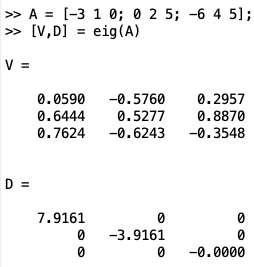
\includegraphics[width=2.5in]{figures/codeQ12_x}

The eigenvectors are the columns of \texttt{V}, and the eigenvalues are the diagonal elements of \texttt{D}.


The determinant of \VA\ is the product of the eigenvalues.
\begin{align*}
	\mathrm{det}(\VA) &= \lambda_1\lambda_2\lambda_3 \\
		&= 7.9161\times-3.9161\times0.0 \\
		&= 0
\end{align*}
 
The matrix \VA\ has a determinant of zero, so it must be rank deficient. Using \Matlab's rank function we see that the rank is only two.
}
\end{question}




\end{document}
